% ********** Chapter 1 **********
\chapter{Java und Skriptsprachen}
\label{sec:javanscripts}
In diesem Kapitel soll zun"achst besprochen werden, welche M"oglichkeiten prinzipiell existieren
um Skriptsprachen wie PHP innerhalb einer Java Virtual Machine auszuf"uhren, und um Daten 
zwischen den beiden Programmiersprachen auszutauschen. Dann werden zwei Technologien vorgestellt,
die in diesem Kontext vorrangig benutzt werden, das \emph{Bean Scripting Framework} und der
\emph{Java Specification Request 233},  und es wird erl"autert welche sich besser f"ur die L"osung 
der Aufgabe eignet. Ausserdem wird erl"autert auf welche Weise PHP in Java integriert
werden soll und es wird ein simpler Prototyp entwickelt, um die Machbarkeit zu erweisen und um erste Erfahrungen
mit der einzusetztenden Technologie zu erlangen. Schlussendlich wird das Projekt in drei Unterprojekte
unterteilt und ein Zeitrahmen f"ur die einzelnen Schritte festgelegt.

\section{Herangehensweisen}
\label{sec:javanscripts:ucs}
Beim Erweitern von Java um die F"ahigkeit Skriptsprachen auszuf"uhren exisiteren zwei wesentliche Anwendungsf"alle:
\begin{description}
\item[Java Objekte in Skriptsprachen:]
Hierbei werden Java-Klassen benutzt um das Leistungsverm"ogen einer Skriptsprache zu erweitern. Die Skriptsprache
soll f"ahig sein Java Objekte zu instanziieren und auf deren "offentliche (public) Methoden und Variablen 
zuzugreiffen. Beispiele f"ur eine solche Integration von Java und einer Skriptsprache sind \emph{Live Connect} von
Netscape und propriet"are APIs der Microsoft Java Implementierungen.
\item[Skripte in Java:]
Java Applikationen soll es m"oglich sein existierende Skripte auszuf"uhren, diesen Skripten Eingabedaten
zur Verf"ugung zu stellen, deren R"uckgabewerte und innerhalb der Skripte vorhandene Daten auszulesen, 
und gezielt auf Funktionen und Methoden eines laufenden Skriptes zuzugreiffen.
\end{description}
Diese beiden Use-Cases enthalten sich zum Teil gegenseitig und teilen sich viele Anforderungen, um sie
zu erf"ullen existieren mehrere Herangehensweisen:
\begin{description}
\item[Java Interpreter:]
F"ur einige Skriptsprachen sind Interpreter erh"altlich die komplett in Java implementiert sind, und welche
meist "uber externe Schnittstellen verf"ugen, was es einer Java-Applikation erlaubt dies einzubetten
und Skripte der entsprechenden Sprache auszuf"uhren. Leider folgen diese Schnittstellen keinem gemeinsamen
Standard, auch weil zum Entwicklungszeitpunkt dieser Interpreter oftmals kein solcher Standard existierte.
Beispiele f"ur diese Art der Einbettung sind unter anderem die Javascript-Implementierung
der Mozilla Foundation \emph{Rhino} und \emph{Jacl}, ein vollst"andig in Java geschriebener Interpreter
f"ur TCL. 
\item["Ubersetzung von Skriptcode nach Java Sourcecode:]
Einige Skriptsprachen verf"ugen "uber Sprachkonstrukte und eine Syntax welche stark an Java angelehnt sind,
daher ist es m"oglich Sourcecode solcher Sprachen in Java-Sourcecode zu "ubersetzen. Allerdings ist das
Entwickeln eines solchen Transcoders "ausserst aufw"andig, so dass es meist einfacher ist Skripte solcher
Sprachen manuell nach Java zu portieren. Beispiele solcher Sprachen sind die BeanShell und Groovy.
\item["Ubersetzung von Skriptcode nach Java Bytecode:]
Es existieren einige Compiler die versuchen Skriptcode direkt in Java Bytecode zu "ubersetzen. Die so
generierten Klassen sind k"onnen direkt von der JVM ausgef"uhrt werden. Das Entwickeln eines solchen
Compilers ist zwar "ahnlich aufw"andig wie das Entwickeln eines oben vorgestellten Transcoders, allerdings
kann die JVM vom Compiler einfach wie eine weitere Hardwareplatform behandelt werden, und da viele
Skriptsprachen schon ausf"uhrbaren Code erzeugen k"onnen muss nur noch die Codegenerierung ausgetauscht,
alle anderen Teile des Compilers, wie syntaktische und semantische Analyse, k"onnen unver"andert weiterbenutzt
werden. Ein Beispiel eines solchen Compilers ist Jython f"ur die Skriptsprache Python. 
\item[Eingebettete, native Interpreter:]
Die wohl einfachste M"oglichkeit eine Skriptsprache in Java einzubetten ist, diese als native Bibliothek mittels
des JNI (siehe \ref{sec:intro:backgroud:JNI}) einzubinden und mit einem Adapter zu umh"ullen (engl. \emph{wrapping}). 
Ein solcher Wrapper wird auch \emph{language binding} genannt.
\end{description}
Eine Softwarekomponente die das Ausf"uhren von Skripten einer bestimmten Sprache erlaubt, und dabei ein standardisiertes
Interface implementiert und somit zumindest in der Theorie austauschbar ist, soll im weiteren Verlauf
dieses Dokumentes \emph{Skriptengine} genannt werden.

Es existieren zwar Ans"atze PHP Interpreter in Java zu implementieren, ein prominentes Beispiel
ist \emph{Quercus} von \emph{Caucho Technology} \cite{CAUCHOHP}. Allerdings gestaltet sich dieses Vorhaben durch
die grosse Menge an PHP "'built-in"' Funktionen, Funktionen also die nicht mittels PHP verwirklich wurden, 
sondern die direkt vom Interpreter erkannt und ausgef"uhrt werden, als sehr schwierig. Diese "'Bibliothek"' wird
auch mit jeder PHP-Version umfangreicher und unterliegt  st"andigen Ver"aenderungen. Desweiteren enthalten solche
Interpreter in aller Regel keine M"oglichkeit PHP-Extensions zu benutzen. Folglich schied diese Art der
Integration von PHP in Java aus, und es musste eine Methode gefunden werden den vorhandenen, originalen PHP-Interpreter
aus Java heraus anzusprechen.

Um PHP in anderen Umgebungen einzubetten bietet es dem Benutzer die M"oglichkeit als dynamisch ladbare
Bibliothek (.dll unter Windows, .so unter unixoiden Betriebssytemen) kompiliert zu werden, Java wiederum
erlaubt das Einbinden solcher Bibliotheken zur Laufzeit mittels des JNI (siehe \ref{sec:intro:background:JNI}).
Um auf den PHP-Interpreter derart zugreiffen zu k"onnen muss eine sogenannte \emph{SAPI} implementiert
werden. SAPI steht in diesem Kontext f"ur "'Server Application Programming Interface"' und ist ein PHP-interner
Begriff. 
Der naive Ansatz PHP innerhalb von Java auszuf"uhren w"are nun das simple Einbinden dieser Bibliothek und
der Zugriff auf Selbige "uber JNI gewesen. Hierzu w"are es aber n"otig gewesen selbst eine Schnittstelle 
zu entwickeln die diesen Zugriff formalisiert, allerdings existierten schon zwei unabh"ngig voneinander entwickelte
Methoden Skriptsprachen innerhalb Javas zu verwenden - das \emph{Bean Scripting Framework} des \emph{Apache
Jakarta Project} und ein sogenannter \emph{Java Specification Request}. So musste evaluiert werden, ob nicht
eine dieser beiden Technologien ein geeigner Weg w"are dieses Ziel zu erreichen. 

\section{Bean Scripting Framework - BSF}
\label{sec:javanscripts:bsf}

Die aktuelle Version 2.4 des Bean Scripting Frameworks - urspr"unglich von IBM entwickelt und nun Teil des
Apach Jakarta Projektes \cite{BSFHP} - bietet eine API, welche es einer Java-Applikation erlaubt 
Skriptsprachen einzubinden und die den derart ausgef"uhrten Skripten den Zugriff auf Java-Objekte der ausf"uhrenden Applikation erm"oglicht.
F"ur jede auszuf"uhrende Skriptsprache wird eine Implementierung des Interfaces \texttt{BSFEngine} ben"otigt, welches eine
Abstraktion der F"ahigkeiten der Skriptsprache darstellt und so der Applikation ein generisches Zugriffschema
auf jegliche Skriptsprache bietet. Alle Instanzen von BSFEngines werden von einer einzigen Instanz der Klasse \texttt{BSFManager} 
verwaltet. Zus"atzlich h"alt dieser ein Register von Objekten (die \emph{object registry}) vor, auf welche der Zugriff aus den 
laufenden Skripten heraus m"oglich sein soll. Der BSFManager h"alt so lange er existiert den Ausf"uhrungszustand aller bei 
ihm registrierten BSFEngines vor, was das Anhalten und sp"atere Fortsetzen eines Skriptes erlaubt.
Das BSF ist in so gut wie allen Jakarta-Produkten wie Ant, Xalan, und Tomcat schon enthalten, so ist es beispielsweise
m"oglich unter Tomcat JSPs in vom BSF unterst"utzten Skriptsprachen zu formulieren.
Zu diesem Zeitpunkt existieren BSFEngine-Implementierung f"ur eine Vielzahl von Skriptsprachen, darunter Javascript/ECMAScript, 
Python, Ruby und XSLT, allerdings keine Implementierung f"ur PHP. Die Dokumentation des BSF ist sehr knapp gehalten, allerdings
beinhaltet sie alle n"otigen Informationen "uber Architektur und Funktionsweise des Frameworks, ausserdem sind alle
Teile des Frameworks unter einer Open Source Lizenz im Quelltext verf"ugbar.

Eine BSFEngine muss folgende Methoden implementieren:
\begin{itemize}
    \item initialize()  - wird zu Begin der Lebenszeit der Skriptengine aufgerufen, um diese zu initialisieren.
    \item call()  - zum Aufruf bestimmter Funktionen oder Methoden innerhalb des in der BSFEngine geladenen Skriptes.
    \item eval()  - mittels eval wird ein als String "ubergebener Ausdruck ausgewertet und ein R"uckgabewert zur"uckgeliefert.
    \item exec()  - mittels exec wird ein komplettes Skript ausgef"uhrt.
    \item declareBean()  - mit dieser Methode wird explizit eine Instanz einer bestimmten Klasse innerhalb der BSFEngine erzeugt.
    \item undeclareBean()  - wird genutzt, um ein vorher mittels declareBean erzeugtes Objekt aus der Engine zu entfernen.
\end{itemize}

Nachdem dieser Wrapper f"ur die gew"unschte Sprache implementiert ist muss die neue BSFEngine beim BSFManager mittels der
Methode \texttt{registerScriptingEngine()} registriert werden. Fortan k"onnen Skripte dieser Sprache mittels der normalen
BSF API ausgef"uhrt werden, hierzu bietet der BSFManager, neben vielen Methoden die auch in einer BSFEngine zu finden sind,
unter anderem folgende Methoden:
\begin{description}
    \item[loadScriptingEngine()] - versucht eine BSFEngine f"ur eine gew"unschte Sprache zu erstellen.
    \item[registerBean()] - f"ugt der object registry ein Objekt hinzu.
    \item[lookupBean()] - gibt ein Objekt aus der object registry zur"uck.
\end{description}
Ausserdem verf"ugt der BSFManager noch "uber methoden mit denen es m"oglich ist Sourcecode und ganze Skripte in sogenannte
\texttt{CodeBuffer} Objekte zu "ubersetzen und erst sp"ater auszuf"uhren.
Das BSF deklariert automatisch innerhalb des ausgef"uhrten Skriptes ein Objekt namens \emph{BSF}, welches den mit der
BSFEngine assoziierten BSFManager repr"asentiert. "Uber dieses Objekt kann aus dem Skript auf Daten und Objekte aus der
Java-Anwendung zugegriffen werden.

\section{JSR 223 - Scripting for the Java Platform}
\label{sec:javanscripts:jsr}

Ein \textbf{J}ava \textbf{S}pecification \textbf{R}equest ist Teil des Java Community Process (JCP), stellt
eine Anforderung den Java Standard (\textbf{J}ava \textbf{L}anguage \textbf{S}pecification - JLS) zu erweitern dar und wird 
normalerweise von einem Expertenteam geleitet.

Der JSR mit der Nummer 223 \cite{JSRHP} beschreibt - "ahnlich dem BSF - Mechanismen welche es Skripten erlauben sollen auf Informationen
innerhalb einer Java-Applikation zuzugreiffen, sowie serverseitige Java-Applikationen dazu bef"ahigen sollen Skriptsprachen f"ur Webseiten 
einzusetzen (\emph{web scripting}). Urspr"unglich wurde JSR 223 zwar explizit f"ur diesen serverseitigen Einsatz von Skriptsprachen 
konzipiert, allerdings wird diese Einschr"ankung in der neuesten Version (Proposed Final Draft, 10 August 2006) relativiert
und auch der Einsatz in anderen Anwendungsgebieten ber"ucksichtigt. In diesem Dokument werden einige Begrifflichkeiten definiert:

Als \emph{scripting engine} wird eine Softwarekomponente bezeichnet, welche in einer Skriptsprache geschriebene Programme ausf"uhrt.
Eine scripting engine beinhaltet normalerweise einen \emph{interpreter} der die eigentliche Ausf"uhrung des Programmes "ubernimmt und
wiederum aus einem \emph{front-end} und einem \emph{back-end} besteht. Das front-end ist f"ur die lexikalische und syntaktische
Analyse des Quelltextes zust"andig und "uberf"uhrt diesen in eine Zwischenform, den sogenannten \emph{intermediate code}.
Das back-end f"uhrt diesen intermediate code aus und nutzt Symboltabellen (\emph{symbol table}) um Variablen innerhalb des Skriptes
zu speichern. Die Spezifikation geht davon aus, dass alle diese Softwarekomponenten Java Objekte sind, wobei explizit erlaubt wird
dass einige dieser Objekte native Aufrufe nutzen. Scripting engines die die \emph{General Scripting API} implementieren werden als 
\emph{Java Script Engines} bezeichnet, eine ob der Existenz einer Programmiersprache gleichen Namens etwas ungl"ucklich gew"ahlten 
Bezeichnung.

Die Spezifikation unterteilt sich in zwei gro\ss e Abschnitte: zun"achst werden \emph{Java Language Bindings} besprochen, Mechanismen
die es Skripten erlauben Java-Klassen zu laden, Objekte zu erzeugen und Methoden dieser Objekte aufzurufen. Im selben Kapitel wird
auch beschreiben wie Methodenaufrufe in Skriptsprachen in Java-Methodenaufrufe umgesetzt, und wie die Argumente und 
R"uckgabewerte dieser Aufrufe zwischen den beiden Sprachen hin- und hergereicht werden. Dieser Teil der Spezifikation ist allerdings
nicht normgebend, da es sehr von den Eigenschaften der Skriptsprache abh"angt wie solche Sprachbindungen realisiert werden m"ussen.
Es werden drei Arten von Language Bindings besprochen: \emph{Dynamic Bindings} werden zur Laufzeit des Skriptes erzeugt, als
\emph{Programmatic Bindings} werden Sprachbindungen bezeichnet die etwa "uber Stellvertreterobjekte innerhalb des Skriptes 
den Zugriff auf Objekte der Java-Anwendung erlauben. Die dritte Art Sprachbindungen werden \emph{Static Bindings} genannt und
beziehen sich auf Funktionen welche die Skriptengine selbst direkt auf Funktionen innerhalb Javas abbildet, so k"onnte beispielsweise
der PHP-Befehl "'\texttt{echo()}"' direkt einen Aufruf der Java-Methode \texttt{System.out.println()} bewirken.
Der zweite grosse Abschnitt besch"aftigt sich mit der \emph{General Scripting API}, einer Sammlung von Interfaces und Klassen, 
welche es erlauben dass Skriptengines als Komponenten in Java-Anwendungen eingebettet werden k"onnen. Diese API unterteilt sich
in einen implementationsabh"angigen und einen Implementierungsunabh"angigen Teil um eine gro"esstm"ogliche Portabilit"at zwischen
verschiedenen Implementierungen zu erreichen. Hierzu ist es notwendig zur Laufzeit Informationen "uber Skriptengines abfragen
zu k"onnen, diese \emph{Metainformationen} beschreiben F"ahigkeiten und Funktionsdetails und werden von jeder Implementierung bereitgestellt.
Dieser Mechanismus zum Auffinden und zum Abfragen von ScriptEngineFactories zur Laufzeit wird im Spezifikationsdokument 
als \emph{discovery mechanism} bezeichnet.
Die wichtigsten Klassen der General Scripting API sind der \texttt{ScriptContext},
die \texttt{ScriptEngine}, die \texttt{ScriptEngineFactory} und der \texttt{ScriptEngineManager}.
\begin{description}
    \item[ScriptContext] - der ScriptContext wird benutzt um einem Skript den Zugriff (engl. \emph{view}) auf Daten der 
    Wirtsapplikation zu erlauben. Dies geschieht mittels Schl"ussel/Wertepaaren, die verschiedenen G"ultigkeitsbereichen
    (engl. \emph{scope}) zugeordnet sind. Die Scopes unterscheiden sich in Sichtbarkeit und Bedeutung. Der ScriptContext 
    bietet den \texttt{GlobalScope}, auf welchen welchen von jeder ScriptEngine aus zugegriffen werden kann die den
    jeweiligen ScriptContext benutzt, und welcher den Zustand der Hostapplikation darstellt.
    Ausserdem bietet der ScriptContext den \texttt{EngineScope}, der nur f"ur eine einzige ScriptEngine g"ultig ist und 
    vorwiegend dazu genutzt wird Variablen innerhalb dieser auszulesen.
    Der Anwender kann jederzeit weitere Scopes definieren, sie werden durch Integerwerte identifiziert. Mittels der
    Methode \texttt{getScopes()} kann der Anwender eine Liste der bekannten Scopes erhalten. Innerhalb der einzelnen Scopes
    k"onnen Werte mittels der Methoden des ScriptContext \texttt{setAttribute()}, \texttt{getAttribute()} und \texttt{removeAttribute()} 
    gesetzt, beziehungsweise abgerufen und gel"oscht werden, dazu ist jeweils der Schl"ussel als String "ubergeben werden muss.
    \item[Binding] - auf Scopes kann mittels des Interfaces \texttt{Bindings} zugegriffen werden. Bindings implementiert
    das Interface \texttt{Map}, mit der zus"atzlichen Anforderung dass alle Schl"ussel nicht-leer und nicht Null sind.
    \item[ScriptEngine] - das ScriptEngine-Interface ist eine Abstraktion eines Skriptinterpreters und muss von
    allen Java Script Engines implementiert werden. Es beinhaltet Methoden um Skripte auszuf"uhren und diesen
    Schl"ussel/Wertepaare zu "ubergeben. Optional kann eine Skriptengine dem Anwender auch die M"oglichkeit bieten
    Skriptquelltexte in intermediate Code zu "ubersetzen und diesen dann wiederholt auszuf"uhren, was allerdings
    vorraussetzt dass die Skriptengine den explizit den Zugriff auf front- und back-end erlaubt. Jede ScriptEngine hat einen
    Standardkontext, der mittels der Methoden \texttt{getContext()} und \texttt{setContext()} manipuliert werden kann. Anstatt den
    Umweg "uber die Scopes zu gehen kann der Anwender einer ScriptEngine Werte auch direkt mittels der Methoden \texttt{get()} und 
    \texttt{put()} "ubergeben, welche sich auf den EngineScope auswirken. Die eigentliche Ausf"uhrung eines Skriptes kann mittels der
    verschiedenen \texttt{eval()} Methoden bewerkstelligt werden, die sich meist nur in der Art und Weise der Quelltext"ubergabe
    unterscheiden.
    \item[Compilable] - Compilable ist ein Interface das optional von einer ScriptEngine implementiert werden kann, wenn sie in der Lage
    ist intermediate Code zu produzieren. Eine solche ScriptEngine bietet die Methode \texttt{compile()} an, welche eine Instanz
    von \texttt{CompiledScript} zur"uckgibt. Ein CompiledScript kann von der ScriptEngine wieder mittels \texttt{eval()} ausgef"uhrt werden.
    Es wird davon ausgegangen, dass CompiledScripts von anderen Aufrufen von eval() nicht beeinflusst werden.
    \item[Invocable] - Invocable ist wie Compilable ein weiteres optionales Interface welches von einer ScriptEngine implementiert
    werden kann. Invocable ScriptEngines bieten dem Anwender die M"oglichkeit Prozeduren, Funktionen und Methoden eines Skriptes 
    direkt aufzurufen, deren Aufruf mittels der Methoden \texttt{invokeFunction()} und \texttt{invokeMethod()} geschieht.
    Die Methode \texttt{getInterface()} liefert eine Instanz einer Java-Klasse zur"uck, welche in der ScriptEngine mittels
    Skriptcode implementiert ist.
    \item[ScriptEngineFactory] - Die ScriptEngineFactory kann genutzt werden um eine ben"otigte ScriptEngine zu erstellen,
    f"ur jede ScriptEngine-Implementierung muss eine korrespondierende Implementierung der ScriptEngineFactory vorhanden sein.
    Hierzu enth"alt sie Methoden um auf die oben beschriebenen Metainformationen zuzugreiffen, zus"atzlich bietet eine ScriptEngineFactory
    die Methoden \texttt{getOutputStatement()}, \texttt{getMethodCallSyntax()} und \texttt{getProgram()} an, mit deren Hilfe
    man Strings erzeugen kann, die von der zugeh"origen ScriptEngine als Skript ausgef"uhrt werden k"onnen.
    \item[ScriptEngineManager] - der ScriptEngineManager hilft dem Anwender ScriptEngineFactories f"ur alle verf"ugbaren
    ScriptEngines zu finden. Hierzu bietet er die Methoden \texttt{getEngineByExtension()}, \texttt{getEngineByMimeType()} und
    \texttt{getEngineByName()}. Mittels analoger \texttt{register...()}-Methoden kann dieser Auffindungsprozess zur Laufzeit
    angepasst werden.
    Zus"atzlich verwaltet er - "ahnlich wie in der BSF der BSFManager - die Kontexte der ihm unterstellten Skriptengines.
\end{description}

Von der Firma Zend existiert eine JSR 223 Referenzimplementation f"ur PHP5, allerdings ist diese nicht im Quelltext verf"ugbar,
und das mitgelieferte PHP erf"ullt wegen fehlender Extensions nicht ganz die Anspr"uche die die Aufgabe stellt.
Der JSR 223 wird Teil der JLS 6 sein, welche vorraussichtlich im Dezember 2006 erscheinen wird.

\section{Ergebnis der Analyse}
\label{sec:javanscripts:fazit}

Sowohl das Bean Scripting Framework, als auch der JSR 223 erwiesen sich als geeignete Technologien, um die gestellte Aufgabe zu 
erf"ullen. Allerdings bot der JSR 223 aus Sicht des Autors einige Vorteile: 
Die verf"ugbare Dokumentation ist - ganz im Gegensatz zur Dokumentation des BSF - sehr umfangreich, vor allem geht sie auch
auf Details wie Methodenaufrufe ein. Die API stellt sich auch etwas kompletter dar, die Interfaces Invocable und Compilable 
helfen Implementierungsunterschiede zu sauber "uberwinden. Auch die Tatsache dass der JSR 223 aller Vorraussicht nach Teil
des Java Standards werden wird sprach, gepaart mit der Unterst"utzung durch namhafte Firmen wie Sun, IBM und vor allem auch 
Zend, eher f"ur als gegen diese Technologie. Die Existenz einer Referenzimplementation f"ur PHP erlaubt nicht nur das
schnelle Entwickeln eines Prototypen, sondern bewies eben auch, dass die Vorgehensweisen welche der JSR 223 vorschl"agt 
gangbar und eine L"osung der gestellten Probleme zumindest im Bereich des M"oglichen lagen, w"ahrend alle verf"ugbaren
Skriptengines f"ur das BSF komplett in Java implementiert waren.
Somit wurde vom Autor gemeinsam mit den Betreuern entschieden dem JSR 223 den Vorzug zu gew"ahren.

\section{Prototyp}
\label{sec:javanscripts:prototype}

Nachdem die Entscheidung "uber die zu verwendete Technologie getroffen wurde musste diese validiert werden. Hierzu wurde
eine Machbarkeitsstudie mit der von Zend zu Verf"ugung gestellten, und kostenlos herunterladbaren Referenzimplementation
f"ur PHP durchgef"uhrt. Es sollte ein einfaches PHP Skript ausgef"uhrt werden, welches trotzdem eine gute Absch"atzung
des Funktionsumfanges des mitgelieferten PHPs erlauben sollte. Um allerdings sicherzustellen, dass zumindest der 
Implementierungsunabh"angige Teil funktioniert wurde ein Programm geschrieben, welches lediglich eine Liste der verf"ugbaren
Skriptengines ausgibt. Hierbei wurde nun festgestellt, dass sich die Referenzimplementation nicht komplett an den Standard
h"alt - so lautet die Signatur der Methode \texttt{getScriptEngineFactories()} des ScriptEngineManagers beispielsweise 
nicht wie von der Spezifikation verlangt
\begin{lstlisting}[name=Vom Standard verlangte Signatur]
    List<ScriptEngineFactory> getScriptEngineFactories()
\end{lstlisting}
sondern
\begin{lstlisting}[name=Signatur in der Referenzimplementation]
    ScriptEngineFactory[] getScriptEngineFactories()
\end{lstlisting}
Dies lies f"ur die weitere Entwicklung unter Zuhilfename der Referenzimplementation schlimmes vermuten.
Als Test f"ur den Implementierungabh"angigen Teil wurde die PHP-Funktion \texttt{phpinfo()} ausgew"ahlt, welche
Text ausgibt, aus dem sich alle geladenen Extensions, sowie alle gesetzten Umgebungsvariablen und 
PHP-Versionsinformationen ersehen lassen. Leider war es dem Autor unm"oglich diesen Protoypen mittels der Zend-Implementierung\footnote{
bezogen "uber \cite{JSRDL}}
zu verwirklichen, da das Laden der mitgelieferten php5.so sowohl und FreeBSD, als auch unter 64- und 32-Bit Linux mit 
verschiedensten Java Versionen zum Absturz der Java Virtual Machine f"uhrte. Die Tatsache dass die Referenzimplementation nicht
im Quelltext verf"ugbar ist verhinderte gleichzeitig die Neu"ubersetzung oder eine effektive Fehlersuche, weiterhin bedeutete
dies eine sehr mangelhafte Kontrolle "uber die benutzte PHP-Version.

Weiterhin existiert neben der Referenzimplementation eine PHP-Extension namens \emph{php/Java bridge}, die das Erzeugen von 
Java-Objekten und das Aufrufen derer Methoden aus PHP heraus erlaubt, siehe hierzu \ref{sec:background:bridge}. 
Allerdings fehlt dieser Extension erstens die M"oglichkeit aus Java heraus gezielt PHP-Funktionen und -Methoden aufzurufen, 
ausserdem verwendet sie nicht das JNI zur Kommunikation zwischen den beiden Sprachen, sondern nutzt ein spezielles XML-Protokoll
um jeglichen Aufruf und jeden Parameter zu serialisieren und "uber lokale Sockets an die JVM zu senden. 
Diese Herangehensweise leidet unter "ahnlichen Problemen wie alle Plattform-agnostischen Protokolle zum Aufruf entfernter Methoden 
im allgemeinen, und XML-basierter Protokolle wie beispielsweise SOAP und XML-RPC im speziellen, siehe hierzu
\ref{sec:background:soap}.

Aus diesen und aus einigen weiteren Gr"unden wurde beschlossen eine eigene JSR 223 Implementierung f"ur PHP zu entwickeln.

\section{Projektplan}
\label{sec:javanscripts:project}

Zu diesem Zeitpunkt waren die zur Durchf"uhrung des Projektes n"otigen Vorarbeiten abgeschlossen, alle n"otigen Informationen waren
gesammelt und die verf"ugbaren Technologien waren evaluiert. Nun sollte ein erster, grober Projektplan erstellt werden, der das Projekt
in seine Teilbereiche unterteilt.
Aufgrund dieser Analyse und der Erfahrungen mit dem Protoypen wurde das Projekt in drei gro\ss e Teilbereiche aufgeteilt:

Zuerst sollte die Ausf"uhrung von PHP Sourcecode innerhalb einer Java Virtual Machine erm"oglicht werden. Hierzu sollte
mittels einer eigenen Implementierung des JSR 223 ein m"oglichst austauschbares PHP verwandt werden k"onnen. 
Ziel sollte hierbei insbesondere die Ausf"uhrung eines m"oglichst grossen Teils des XP-Frameworks sein. Als Ergebnis sollte 
am Ende ein einfach zu benutzendes Java-Archiv, zusammen mit einigen Funktionstests entstehen, das dann in weiteren Teilprojekten 
eingesetzt werden konnte. Fuer diesen Teil des Projektes wurden sechs Wochen veranschlagt.

Im zweiten Teilprojekt sollte der Einsatz von PHP innerhalb eines Java Application Servers - beispielsweise JBoss - erforscht
und vereinfacht werden. Grossen Wert sollte hierbei auf ein m"oglichst einfaches Ausbringen (\emph{deployment}) derart 
entwickelter Anwendungen gelegt werden. Hierzu sollte auch die Notwendigkeit Java-Quelltext zu schreiben auf ein Minumum reduziert, 
oder wenn m"oglich komplett eliminiert werden. Hierf"ur wurden weitere zwei Wochen eingeplant.

Vier Wochen sollten darauf verwandt werden m"oglichst viele Eigenschaften des JavaEE Application Servers
f"ur die ausgef"uhrten PHP-Skripte erreichbar zu machen. Dazu z"ahlen die Persistenzanbindung, beispielsweise mittels Java
Persistance und besonders die Anbindung an JMI, zum Beispiel als Message Driven Bean.

Schlussendlich sollte die restliche Zeit genutz werden um die Ausarbeitung fertigzuschreiben, und um Dokumentation "uber die
Bibliothek und das Aufsetzen einer Beispielumgebung zu erstellen. Diese Zeit war auch als Puffer f"ur eventuell auftretende
Probleme zu verstehen.

Im Laufe der Entwicklung der JSR 223 Implementierung wurde jedoch festgestellt, dass zus"atzlich zum reinen Ausf"uhren von PHP-Skripten
innerhalb einer Java-VM noch einiges weitere an Funktionalit"at zu realisieren war. Zum einen sollte aus dem PHP-Skript heraus das Erzeugen
von Java-Objekten und der Zugriff auf deren Methoden und Attribute m"oglich sein, und zum anderen sollte auch umgekehrt aus Java heraus ein
Zugriff auf Funktionen und Methoden innerhalb des ausgef"uhrten PHP-Skriptes erm"oglicht werden.

Aus diesem Grund wurde der Projektplan umgestellt, um der JSR 223-Implementierung mehr Zeit einzur"aumen. Hierzu wurden die Forderungen nach
einem Buildsystem f"ur PHP-EJBs komplett gestrichen, und der JBoss- mit dem eigentlichen EJB-Teil zusammengelegt. Dies lie\ss acht Wochen
Zeit um die JSR 223 Implementierung zu erstellen, und vier Wochen um diese in einem JBoss anzuwenden um Session Beans und Message Driven
Beans in PHP zu schreiben und auszuf"uhren. 

Abbildung \ref{fig:plan} zeichnet die Unterteilung des urspr"unglichen und des tats"achlichen Projektplanes "uber die Zeit auf.

\begin{figure}[h]
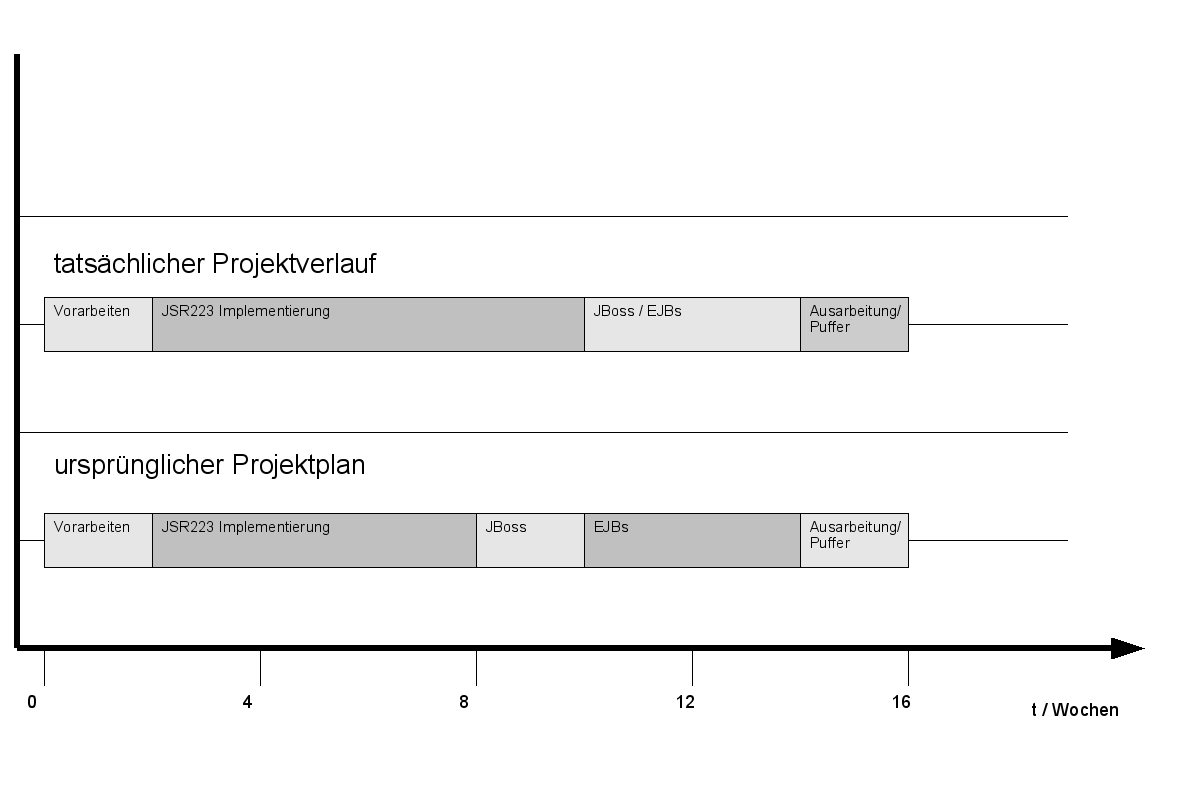
\includegraphics[width=\textwidth]{javanscripts/img/plan.png}
\caption{Projektplan}
\label{fig:plan}
\end{figure}



% ********** End of chapter **********
